\documentclass[12pt, twoside]{article}
\usepackage[letterpaper, margin=1in, headsep=0.5in]{geometry}
\usepackage[english]{babel}
\usepackage[utf8]{inputenc}
\usepackage{amsmath}
\usepackage{amsfonts}
\usepackage{amssymb}
\usepackage{tikz}
\usepackage{yhmath}
%\usetikzlibrary{quotes, angles}

\usepackage{graphicx}
\usepackage{enumitem}
\usepackage{multicol}

\usepackage{fancyhdr}
\pagestyle{fancy}
\fancyhf{}
\renewcommand{\headrulewidth}{0pt} % disable the underline of the header

\fancyhead[RE]{\thepage}
\fancyhead[RO]{\thepage \\ Name: \hspace{3cm}}
\fancyhead[L]{BECA / Dr. Huson / 10th Grade Geometry\\* 7 February 2020}

\begin{document}
\subsubsection*{8.9 Do Now: The equation for a circle}
 \begin{enumerate}

  \item A circle centered at the origin includes the point $P(4,2)$, as shown below.
  \begin{multicols}{2}
    \raggedcolumns
    \begin{enumerate}
      \item Find the radius of the circle. Simplify the radical. \vspace{2.7cm}
      \item Find the point on the circle on the same diameter as $P$.
    \end{enumerate}
      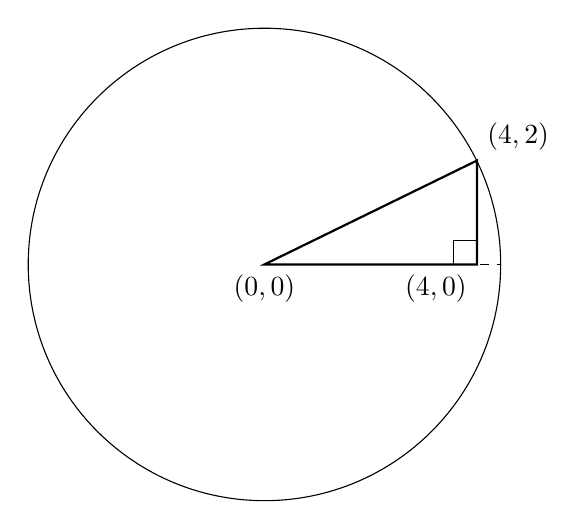
\begin{tikzpicture}[scale=.6]
        \draw (0,0) circle[radius=5];
        \draw [thick]
        (4.5,0) node[below left] {$(4,0)$}--
        (0,0) node[below] {$(0,0)$}--
        (4.5,2.2) node[above right] {$(4,2)$}--cycle;
        \draw [dashed] (0,0)--(5,0);
        \draw (4.5,0) ++(-0.5,0)--+(0,0.5)--+(0.5,0.5);
      \end{tikzpicture}
  \end{multicols}

  \item What is the equation of a circle with center $(3,-2)$ and radius $r=4$. Use the equation $(x-a)^2+(y-b)^2=r^2$. \vspace{1.5cm}
  
\subsubsection*{Algebra competencies}
\item Expand each binomial-squared expression to the form $ax^2+bx+c$.
  \begin{multicols}{2}
  \begin{enumerate}[itemsep=3cm]
    \item $(x-5)^2$ 
    \item $(y+7)^2$ 
  \end{enumerate}
  \end{multicols}\vspace{3cm}
  
  \item Simplify each radical.
  \begin{multicols}{2}
    \begin{enumerate}[itemsep=2cm]
      \item $\sqrt{12}$ 
      \item $\sqrt{40}$
    \end{enumerate}
    \end{multicols}\vspace{2cm}

\newpage
\subsubsection*{Early Finishers: Using the distance formula to prove a parallelogram}
  \item In this problem use the following theorem (copy it at the bottom of the page after your calculations): \\*[0.25cm]
  \emph{A quadrilateral is a parallelogram if and only if it's opposite sides are congruent.}\\*[0.5cm]
  Shown below is quadrilateral $ABCD$, $A(2,-1)$, $B(6,-2)$, $C(8,4)$, and $D(4,5)$. \\*[0.25cm]
  Prove it is a parallelogram by
  \begin{enumerate}
    \item finding the length of each of the four sides,
    \item stating which sides are congruent,
    \item copying the theorem as your conclusion.
  \end{enumerate}
  \begin{flushright} %4 quadrant regents grid
    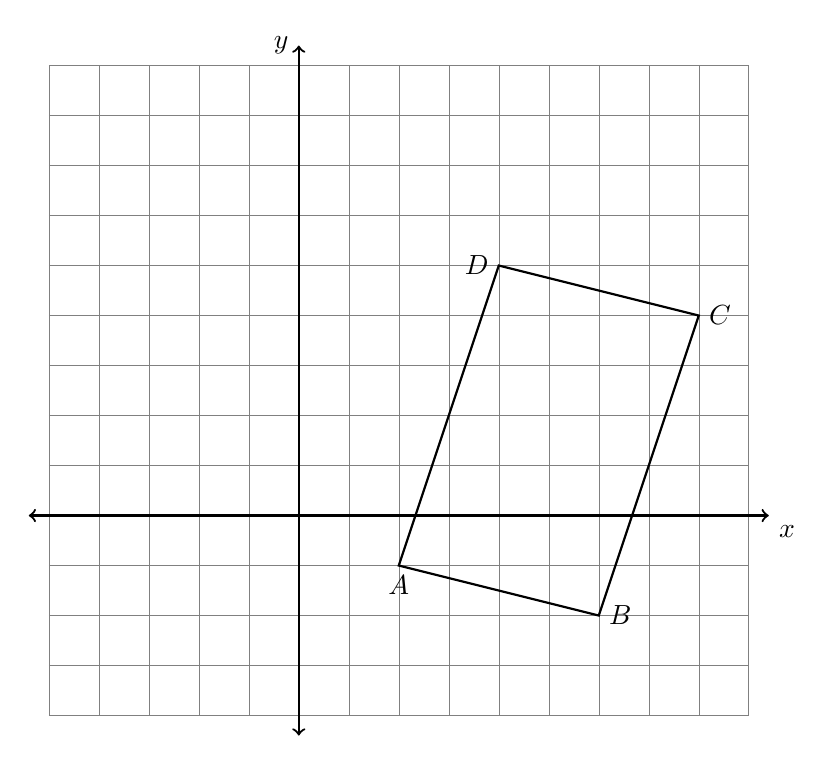
\begin{tikzpicture}[scale=.635]
      \draw [help lines] (-5,-4) grid (9,9);
      \draw [thick, <->] (-5.4,0) -- (9.4,0) node [below right] {$x$};
      \draw [thick, <->] (0,-4.4)--(0,9.4) node [left] {$y$};
      \draw [thick] (2,-1) node[below] {$A$}--
      (6,-2) node[right] {$B$}--
      (8,4) node[right] {$C$}--
      (4,5) node[left] {$D$}--cycle;
    \end{tikzpicture}
  \end{flushright}


\end{enumerate}
\end{document}
